% Voor Engelse tekst, gebruik de optie english achter documentclass.
\documentclass{uvamath}
\usepackage[dutch]{babel}

\usepackage{graphicx}
\usepackage[pdfborder={0 0 0}]{hyperref}

\title{Lossless Image Coding}
\author[chrisz@science.uva.nl, 6127901]{Jolien Kerssens}
\author[jolienk@science.uva.nl, 6123102]{Chris Zaal}
%\author[ingrid@science.uva.nl, 6123102]{Ingrid de Vries}

\what{Verslag Computeralgebra/\LaTeX} % voorbeeld
\supervisors{dr.\ Chris Zaal, Jolien Kerssens}
\secondgrader{}

%\coverimage{\rule{9cm}{9cm}\\\emph{Voeg een plaatje in.}}
\coverimage{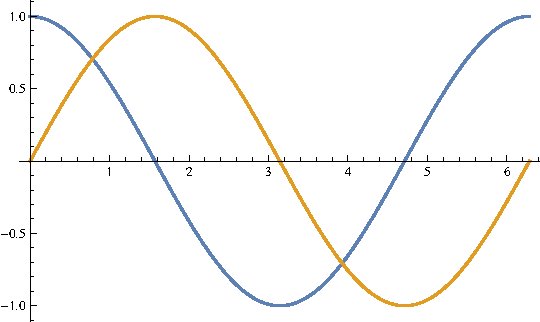
\includegraphics[scale=1.2]{SinCosPlot}}


\begin{document}
\maketitle

\begin{abstract}
Hier een korte samenvatting: over het vak, je project, welk artikel, vraagstelling, hoe onderzocht, wat kwam er uit?
\end{abstract}

\tableofcontents

\chapter{Inleiding}
Hier de inleiding van je verslag: iets over het vak Computeralgebra/\LaTeX, project. Over je artikel: het artikel dat we gekozen hebben, is een artikel over speltheorie: \emph{Average Lenghts for the Two-Player Name Game} \cite{artikelNeal}. Motivatie van je keuze: waarom dit artikel?

Misschien heb je ook nog wel een ander artikel erbij gehaald, waarin ook iets nuttig stond, bijvoorbeeld \cite{artikelHopkins}.

\section{Vraagstelling}
Na lezing van het artikel en discussie (onderling en met de docenten) zijn we tot de volgende vraagstelling gekomen. 


\chapter{Mathematica}
Over de aanpak van de probleemstelling in Mathematica. 

\section{Programma's}
Iets over de code die je geschreven hebt. 

\section{Resultaten}
Wat rolt er uit jullie programma's. 

\chapter{Conclusie}
In dit hoofdstuk rol je alles op: wat zeggen jullie resultaten over jullie probleemstelling? Heb je alles opgelost? Is er meer dat je eventueel nog zou willen oplossen?


\begin{thebibliography}{x}
% Zet dit dit hoofdstuk in de inhoudsopgave.
\addcontentsline{toc}{chapter}{Bibliografie} 

\bibitem{artikelNeal}
  Neal, D. K.,
  \emph{Average Lenghts for the Two-Player Name Game},
  The Mathematical Gazette, \textbf{91}, 520,
  2007.

\bibitem{artikelHopkins}
  Hopkins, D.,
  \emph{Probabilities for the Name Game},
  The Mathematical Gazette, \textbf{77}, 479,
  1993.

\end{thebibliography}

\appendix

\chapter{Mathematica-code}
Hier kun je eventueel de Mathematica-code van je project neerzetten. Mag, maar hoeft niet. 

\chapter{Data}
Hier kun je eventueel (een gedeelte van) je Mathematica-output neerzetten. 

\end{document}